\begin{figure}[!t]
	\centering
	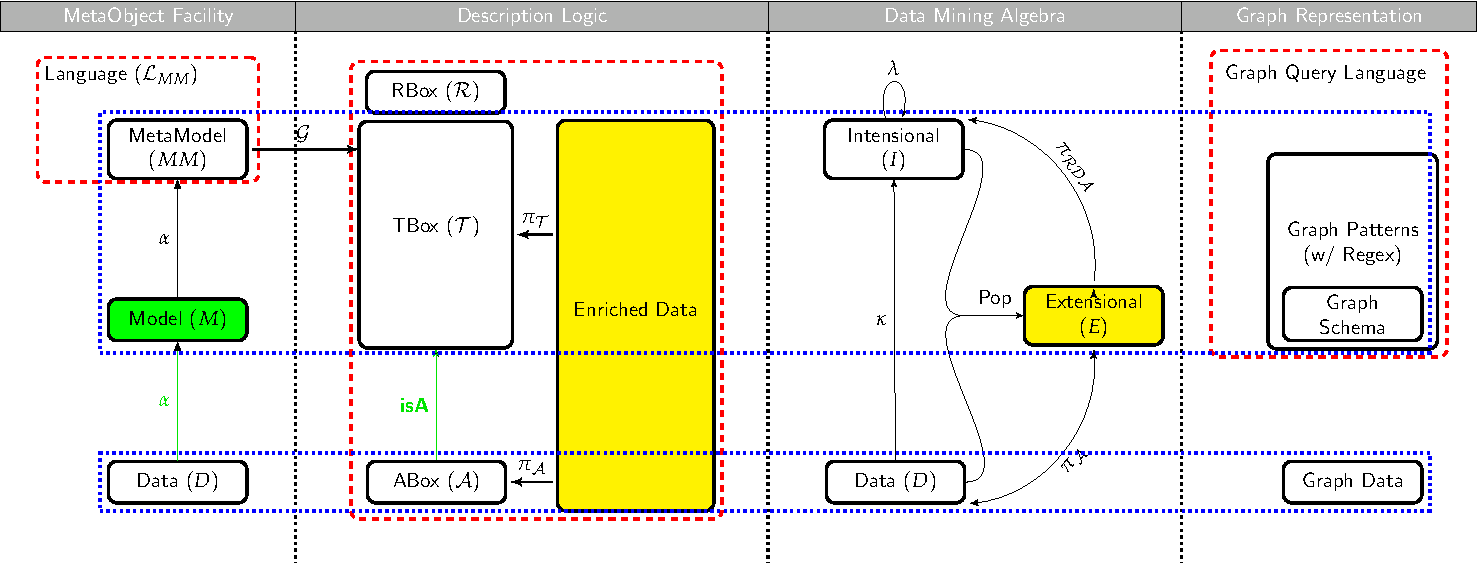
\includegraphics[width=\textwidth]{fig/02models/taonta}
	\caption{A coarse view of all the query languages that have been analysed so far. Red dashed lines represent the level at  which the query languages lie with respect to the representation of the data to be queried. Blue dotted lines represent the level at which either data (below) or its properties (above) are represented.}
	\label{fig:taonta}
\end{figure}
\section{Conclusions}

Structured and semistructured
models point out that a schema can be externally represented, and that (semi)structured data can be represented without the constraints provided by a specific schema, thus allowing a more flexible approach to data integration between different representations. Moreover, the analysis of unstructured data revealed that their translation into a representation of choice depends on a specific scenario, similarly to the adoption of a specific schema to semistructured data.
On the other hand, all the non-graph model fail to represent explicit relations between different data and are all affected by semantic overloading: this last problem will be solved by the property graph model. Additionally, these data model representations failed to provide structural aggregations: the only model achieving this final result was the stream data model: summarized representation is directly associated to the finer values, and each value may be also contained in multiple possible coarser representations. As a consequence, a proper model extending both the semistructured data representation and the graph model is required: chapter \vref{cha:graphsdef} is going to propose GSMs where associations between attribute and value for each tag, tuples and objects are going to be generalized into a \texttt{MultiMap} of object references instead of a single \texttt{Map}; GSMs will also enable structured aggregations.

Finally, we completed the analysis of several types of query languages: those are roughly subsumed by Figure \ref{fig:taonta}. \textcircled{\raisebox{-.5pt}1} At the very beginning of this thesis, we were trying to find a valid  representation of semi-structured data, and recognized that the data model itself shall contain a subset $MM$ of the whole query language $\mathcal{L}_{MM}$. Still, at this abstraction level it was not clear which query language should have been used. Then, \textcircled{\raisebox{-.5pt}2} we analysed the Description Logic framework (Definition \vref{def:dlonta}), which is currently used for data integration, and we observed that, even though this language can be used to model data alongside its properties, it fails to reproduce data transformation operations. Then, we moved to an  \textcircled{\raisebox{-.5pt}3} relational algebra extension for data mining (Section \vref{subsec:dmalgebra}), where it was also possible to transform the tuples' representations and to perform aggregations. Nevertheless, this query language showed the impossibility one singe relational representation for both data and intensional data properties, thus requiring the explicit definition of extra-world operations. Then, we moved to analyse \textcircled{\raisebox{-.5pt}4} graph query languages: we  introduced graph grammars, thus allowing to introduce the pattern matching and rewriting process that happens in proper graph query languages; such operation will allow to both represent most of the possible operations over graph data structures and perform schema alignments and rewritings. We also observed that their instance-specific head rules must be substituted with more general graph pattern matching or traversing queries, thus allowing to nest vertex and edge properties within graph data structures. This observation also suggests that graph data and graph schemas/patterns may be represented using the same data model, thus suggesting that a generalized graph data model should be also able to embed metamodel information. Consequently, we expect that the GSQL query language (Chapter \ref{cha:NGQL}) on top of GSM will also be able to express all the previous queries, as well as embed the GSM's metamodel within its operators.


%We also observed that graph data, similarly to a semistructured data model, allow to uniformely represent data and schemas within the same representation. 
